%!TEX root = ../main_wo_rep.tex
%
% 原子スペクトルの観察
%


\section{原子スペクトルの観察}

\subsection{はじめに}

単一の原子からなるガスを高温に熱したり、高電圧をかけて放電させたりすると特定の波長を持った光を
発します。
この原子が発する光を詳しく調べる事で原子%の定常状態
が持つエネルギーを知ることができ、
原子の構造や量子論の理解へと発展していきました。
この実験では回折格子を利用した簡易分光計を組み立て、様々な原子が発する光の波長を測定し、原子の持つ
定常状態のエネルギーが離散的である事を確認しましょう。

\subsection{原子が発する光}

単一の原子からなる希薄なガスをガラス管に封入し、高電圧をかけるとガス中で放電が起きて
原子が発光します。この光は封入されている原子特有の波長をもっており、原子の種類で見た目の色が異なります。
例えば、トンネルの中などで使われているナトリウムランプは黄色い光を発し、街灯などに使われている
水銀灯は青白い光を発しています。

この原子が発する光を分光計と呼ばれる装置で詳しく調べると、様々な波長を持った光の集まりである事が
わかりますが、太陽光のような連続のスペクトルではなく特定の波長の光だけが明るい輝線として現れた離散的(とびとびの)スペクトルになっています。

\begin{wrapfigure}[14]{r}{8cm}
\vspace*{-0.8cm}
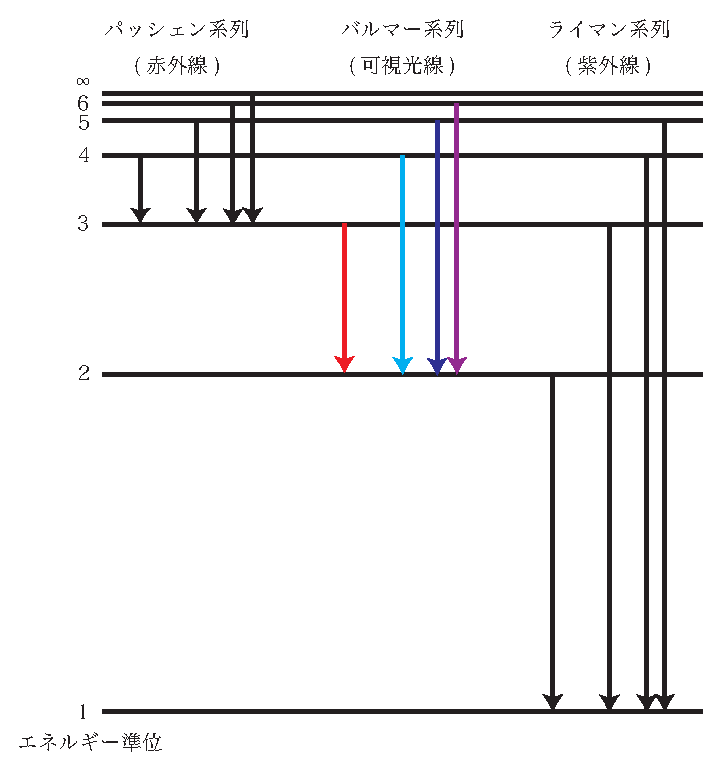
\includegraphics[scale=0.65]{12_Spectrum/state.eps}\\
\hspace{0.5cm}{\small 水素原子のエネルギー準位とスペクトル}
\end{wrapfigure}


これは発光の原理が、ある原子のエネルギーが高い状態から別のよりエネルギーの低い状態へ移るときに、
そのエネルギーの差を光として放出する事に起因しています。量子論の考え方を用いると、原子の定常状態の
エネルギーはある特定の値のみをとることができる離散的なものになります。したがって、ある定常状態から
別の定常状態へ移るときのエネルギーの差も離散的なものとなり、そのエネルギーに応じて
原子が発する光の波長も特定の離散的な値だけになるのです。

原子が2つの定常状態の間を遷移したときのエネルギー差を$\Delta E$とすると、その時に発する光(光子)の振動数$\nu$や波長$\lambda$の間には
\begin{equation}
\Delta E=h\nu=h\frac{c}{\lambda}
\label{Planck}
\end{equation}
の関係があります。ここで、$c$は光の速さ
\[
c = 3.00 \times 10^{8} \quad \text{[m/s]}
\]
で、比例定数$h$はプランク定数とよばれ
\[
h = 6.63 \times 10^{-34} \quad \text{[J$\cdot$s]}
\]
という値です。
原子の励起状態を移り変わるときの
原子の励起状態のエネルギーを扱う場合にはエネルギーの単位としてジュール[J]ではなく、
電子一個が1 [V]の電位差で得るエネルギーを単位とした「電子ボルト[eV] ($=1.60218\times 10^{-19}$ [J])」を用いる方が便利ですので、
以下ではプランク定数をジュールから電子ボルトに換算した
\[
h = 4.14 \times 10^{-15} \quad \text{[eV$\cdot$s]}
\]
を用いる事にします。

%らに、光の振動数$\nu$と波長$\lambda$の間には、光の速さ
%\[
%c = 3.00 \times 10^{8} \quad \text{[m/s]}
%\]
%$\nu=\frac{c}{\lambda}$の関係があるので、

\subsection{簡易分光計の原理}

この実験では原子が発する光のスペクトルを調べるのに簡易的な分光計を組み立てそれを用いる事にします。
一般的な分光計はプリズムを用いて分光しますが、実験で用いる分光計は回折格子を用いています。
回折格子はガラス板やプラスチックフィルムに細かい溝が刻んであり、回折と干渉を利用して光を波長ごとに
特定の角度方向に分光します。

\begin{wrapfigure}[10]{r}{7cm}
\vspace*{-0.8cm}
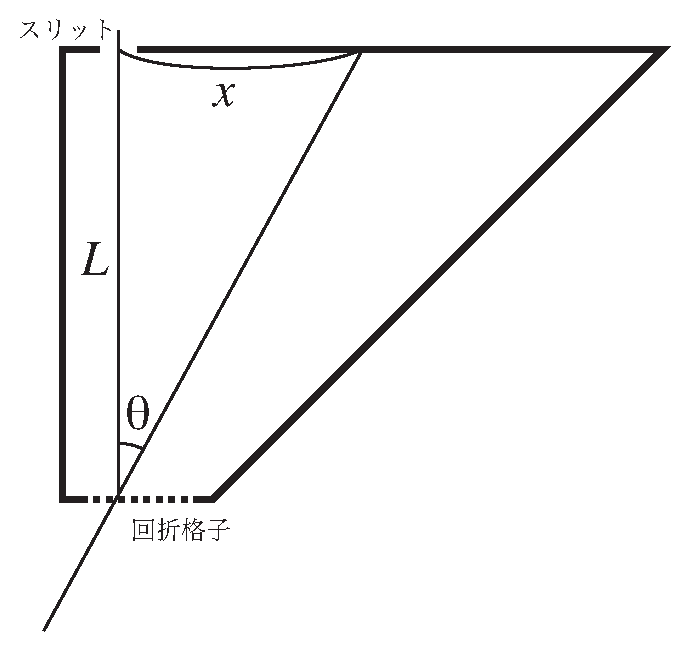
\includegraphics[scale=0.6]{12_Spectrum/spectroscope.eps}
\end{wrapfigure}


実験で用いる簡易分光計の構造は右図の様になっていて、回折格子レプリカフィルムという
1mmにつき500本という細かい溝が刻まれたフィルムを通してスリットからの光を見る事で分光した光を見る事ができます。
スリットとフィルムの位置と光の像が見える位置のなす角度を$\theta$とすると、波長$\lambda$の光が回折格子によって強め合うための条件は
\[
d \sin \theta = n \lambda \qquad (n=1,2,3,\ldots)
\]
で、$d$は回折格子の格子間隔です。実際に観測される明線は$n=1$のみなので、以下では$n=1$とします。

実際の実験では回折格子フィルムから見える目盛りを用いてスリットから輝線までの距離$x$を測定します。
スリットから回折格子までの距離を$L$とすると、
\[
\sin \theta  = \frac{x}{\sqrt{x^2+L^2}}
\]
となるので、$x$の位置に見えた輝線の光の波長は
\[
\lambda = \frac{d x}{\sqrt{x^2+L^2}}
\]
と求まります。(レーザー光を用いた光の干渉実験と異なり$x$と$L$が同程度の大きさなので、ここでは近似が使えません。)

組み立てキットの簡易分光計では$L=26~\text{[cm]}$、$d=\frac{1}{500}~\text{[mm]}$になっているので、$x$を[cm]単位で測った場合、波長は
%\[
%\lambda = \frac{x}{\sqrt{x^2+100}}\times 10^{-4} ~\text{[cm]}
%= \frac{x}{\sqrt{x^2+100}}\times 10^{3}  ~\text{[nm]}
%\]
\begin{eqnarray}
\lambda &=& \frac{x}{\sqrt{x^2+676}}\times 2\times10^{-4} ~\text{[cm]}\nonumber\\
&=& \frac{2x}{\sqrt{x^2+676}}\times 10^{3}  ~\text{[nm]} \nonumber
\end{eqnarray}
という計算で求めることができます。
さらに、関係式(\ref{Planck})を用いると、上の[nm]を単位とした波長に対応するエネルギーは
\[
E=\frac{1.24 \times 10^{3}}{\lambda} ~\text{[eV]}
\]
と求まることになります。

\begin{itembox}[l]{\bf コラム:フラウンホーファー線}

太陽光線を分光器にかけて詳しく眺めると、連続的なスペクトルの中に多数の暗線が混ざっていることがわかる。
この暗線を発見者にちなんで、フラウンホーファー線と呼ぶ。暗線の存在は、対応する波長の光が地表にやってこないことを意味する。なぜ、ある特別な波長の光は地球にやってこないのだろう?

この実験では、原子はエネルギー準位の差に等しい大きさのエネルギーを持った光を放出してエネルギーの低い定常状態に移ることを調べたが、逆にエネルギー準位の差に等しい大きさのエネルギーを吸収するとエネルギーの高い定常状態に移ることができる。太陽の表面で作られた太陽光線は本来連続スペクトルであるが、主に太陽の彩層に存在する原子がその原子に特徴的な波長の光を吸収するので、その波長の光の量が減少して暗線となるのである。
%スペクトルを調べることによって、太陽にどのような元素が存在するのかを調べることができる。実際に、ヘリウムという元素は地球上で見つかる前に太陽に存在する元素としてスペクトルの分析により発見された。
恒星などの天体のフラウンホーファー線の波長は理論的に予言できるため、遠くの星のスペクトルに含まれるフラウンホーファー線のドップラー効果による理論値からのずれを調べると、地球とその天体との相対速度も知ることができる。

\end{itembox}

\newpage

\jikken

\begin{itemsquarebox}[c]{\bf 実験用具}
簡易分光計組み立てキット、原子スペクトル光源(ナトリウム、カドミウム、水銀)、
セロテープ、カッター、カッターマット、スティックのり
\end{itemsquarebox}

\bigskip

\subjikken{簡易分光計の組み立てと原子スペクトルの観察}

\begin{enumerate}

\item 簡易分光計組み立てキットの説明に従い、簡易分光計を組み立てます。\\
※ スケールの目盛りがスリットからの距離を正確に表すように、スケールの取り付けなどは正確に組み立てます。(スリットをふさがないようにスケールの0の端をスリットに合わせて貼ります。)\\
※ 回折格子シートは格子方向がスリットと平行になるように貼付けます。\\
※ 特にスリット穴は分光計の性能に影響するので、丁寧にきれいな穴を開けましょう。

\item ナトリウム管、カドミウム管、水銀管をセットした光源装置から出る光を簡易分光計を用いて観察します。(ランプの色と明るさは点灯して十分時間がたたないと安定しないので注意します。また、ランプを長時間直視しないようにしましょう。)

\item 各ランプのスペクトルの輝線の色と位置を目盛りを使って読み取り記録します。そのとき、目の位置は常にスリットの正面になるよう気をつけましょう。

\item 輝線の位置から輝線の波長を求めます。また、波長から対応するエネルギーを計算します。

\item 白熱灯や蛍光灯についても同様にスペクトルを観察し、その特徴について考えてみましょう。


\end{enumerate}

\newpage

参考:可視部の主なスペクトル線の波長(理科年表より)\\
\hspace*{1cm}
\begin{tabular}{|p{2.0cm}|p{2.0cm}|p{2.0cm}|}
\hline
カドミウム & 水銀 & ナトリウム \\
\hline\hline
643.84696 & 690.716& 589.592 \\
\hline
508.582 & 579.065 & 588.995 \\
\hline
479.992 & 576.959 & \\
\hline
467.815 & 546.074 & \\
\hline
& 435.835 & \\
\hline
& 434.750 & \\
\hline
& 407.781 & \\
\hline
& 404.656 & \\
\hline
\end{tabular}\\
\hspace*{6.0cm}(単位:[nm])

